\appendix

% ===============================================
% ===============================================

\section{Is this specific to ViT image models?}
\label{sec:more_image_architectures}

No.
In the main paper, we only used ViT models for all experiments. Could it be that \lit only works with ViT models, or is in some way specific to the Transformer architecture?

In order to verify that this is not the case, we applied the same recipe to comparably-sized models of different families. Table~\ref{table:more_image_architectures} shows the zero-shot performance with \lit on the CC12M dataset for ViT~\cite{vit}, Mixer~\cite{mixer}, and ResNet~\cite{bit}; all pre-trained on ImageNet21k. Following~\cite{efficiency_misnomer}, we report parameter count, inference speed, and FLOPs to indicate our attempt to match the “model size”. The results show that \lit works for different model families, but also confirm the finding of~\cite{clip} that ViT models do seem more amenable to learning image-text mappings than other architectures of similar size.

\begin{table}[h]
  \newcolumntype{C}{>{\centering\arraybackslash}X}
  \newcolumntype{R}{>{\raggedleft\arraybackslash}X}
  \setlength{\tabcolsep}{0pt}
  \setlength{\extrarowheight}{5pt}
  \renewcommand{\arraystretch}{0.75}
  \centering
  % Format is type{width}, p: paragraph, top-align, C is custom, c is squeezed.
  \begin{tabularx}{\linewidth}{p{1.7cm}p{0.1cm}Cp{0.1cm}Cp{0.1cm}Cp{0.1cm}Cp{0.1cm}Cp{0.2cm}Cp{0.1cm}C}
    \toprule[1pt]
     \bf{Model} &&
    {\centering \rotatebox{90}{\bf{0shot}}} &&
    {\centering \rotatebox{90}{\bf{Adapt}}} &&
    {\centering \rotatebox{90}{\bf{I$\rightarrow$T}}} &&
    {\centering \rotatebox{90}{\bf{T$\rightarrow$I}}} &&
    {\centering \rotatebox{90}{\bf{Param}}} &&
    {\centering \rotatebox{90}{\bf{Speed}}} &&
    {\centering \rotatebox{90}{\bf{FLOPs}}} \\
    \midrule
   ViT-B/32 &&  60.7 &&  79.1 &&  41.3 &&  25.0 && 197\,M &&  2855 && 12\,G \\
 Mixer-B/32 &&  57.1 &&  75.9 &&  37.5 &&  22.9 && 169\,M &&  4208 && \phantom{0}9\,G \\
   BiT-M-R50 &&  55.2 &&  77.6 &&  37.3 &&  23.9 && 134\,M &&  2159 && 11\,G \\
    \bottomrule[1pt]
  \end{tabularx}
  \caption{\protect\lit with different model families. Showing zero-shot top-1 accuracy on ImageNet in comparison to fine-tuning (column “Adapt”). Inference “Speed” is in images per second per core.}\label{table:more_image_architectures}
\end{table}

% ===============================================
% ===============================================

\section{Larger model capacity yields better results}
\label{sec:model_capacity_impact}

\begin{figure}[b]
    \centering
    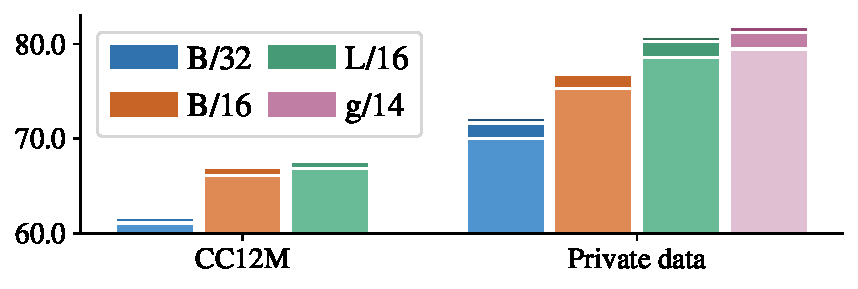
\includegraphics[width=0.48\textwidth]{images/model_capacity_impact.pdf}
    \caption{ImageNet zero-shot accuracy [\%] with varying model capacity. Incremental improvemments due to larger \textit{text} towers (base $\rightarrow$ large $\rightarrow$ huge) are shown as stacked bars.}
    \label{fig:model_capacity_impact}
\end{figure}

Increasing the model capacity of the pre-trained image-tower improves zero-shot ImageNet accuracy more than increasing the capacity of the text-tower.
Figure~\ref{fig:model_capacity_impact} shows substantial gains in the private data setup when the image tower capacity is increased from B/32 and base text tower (74.5\%) to g/14 and huge text tower (81.2\%). We take the pre-trained image towers from~\cite{vitg}, and the text towers were trained from scratch.

The improvements in the public CC12M data setup range from 61.1\% with a B/32 image tower and base text tower up to 67.6\% with the L/16 model combined with a large text tower. In this setup, we used pre-trained BERT text towers~\cite{bert} and pre-trained image models from~\cite{augreg} (using the “recommended checkpoints”). Note that in this case the increase from B/16 to L/16 is more modest (from 66.9\% to 67.6\% with the large text tower), and we see a similar improvement in ImageNet zero-shot performance when increasing the text tower size. 

% ===============================================
% ===============================================

\section{Tuning details on our dataset}
\label{appendix:our_details}
We use the pre-trained transformer models from~\cite{vitg}.
ViT-B/32 was used for most of the ablation tests,
and the larger ViT-B/16, ViT-L/16 and ViT-g/14 models are used in Section~\ref{sec:model_capacity_impact} for capacity impact evaluations.
For our best \Lu results, we adopt the ViT-g/14 model pre-trained in~\cite{vitg}.

During contrastive-tuning, we use the AdaFactor optimizer~\cite{adafactor} following~\cite{vitg}.
We use $0.001$ learning rate, and the default $\beta_1=0.9$ and $\beta_2=0.999$ for AdaFactor optimizer.
We use batch size $16384$ by default, unless otherwise noted.
Input image is simply resized to $224\times224$ resolution (apart from $288\times288$ resolution for “g/14*” model).
No weight decay is used during tuning.
We use cosine learning rate schedule with a linear learning rate warmup of 10k steps.
We train our models for 55k steps by default, which equals to about 900 million seen image-text pairs during tuning. 
For our best runs, we scale up the training schedule to 18 billion seen image-text pairs.
We use 128 TPU cores by default for the above experiments, and 256 TPU cores for our best run with 18 billion seen image-text pairs.


In the \Lu setup, we do not attach the optional linear head on the image tower. 
We observe a very small quality improvement without using the image linear head, thus we remove it for simplicity.

\section{Tuning details on CC12m}
\label{appendix:public_details}

We use pre-trained ViT models from~\cite{augreg} (unless otherwise noted, we used the “recommended checkpoints” from that repository). On the text side, we use BERT-base and BERT-large from~\cite{bert} for most experiments. In section~\ref{sec:more_text_models} we use T5-base from~\cite{T5} and mT5-base from~\cite{mt5}.

We use the Adam optimizer ($\beta_1=0.9$, $\beta_2=0.999$) for all models, except for models with Large text tower that were trained with a modified version of AdaFactor from~\cite{vitg} (same settings as described in Section~\ref{appendix:our_details}).
The learning rate is set to $0.001$, and the weight decay to $0.0001$ (using “decoupled” weight decay as described in~\cite{decoupled}). Gradients are clipped at global norm 1.

For training, the images are pre-processed by Inception-style cropping~\cite{inception} to a size of 224 pixels. For evaluation, the images are resized to 224 pixels with bi-linear interpolation without cropping.

When tuning on the CC12M dataset, we train for 20 epochs (200 million seen image-text pairs), which corresponds to 12k steps with a batch size of 16384. The first 50k image-text pairs are used as minival validation set.
The learning rate is ramped up linearly for the first 2k steps and then follows a cosine decay.
Unless otherwise noted, we use the \LU setup with a linear head on the text tower only.


% ===============================================
% ===============================================

\section{How to use YFCC100m?}
\label{appendix:yfcc}

This section is an exploratory analysis of the YFCC100m dataset and provides guidance on what is a good setup for \lit.
For each experiment we run, we try three learning-rates (0.001, 0.0008, 0.0003) and two weight-decays (0.0001 and 0.00001) and report the best result, this allows avoiding biasing conclusions due to sub-optimal hyper-parameters.
We perform the exploration using the small ViT-B/32 AugReg~\cite{augreg} image tower and a BERT base~\cite{bert} text tower and run tuning for 60\,000 steps, although the same conclusions and similar scores are already reachable after 30\,000 steps of tuning.

\begin{figure}[t]
    \centering
    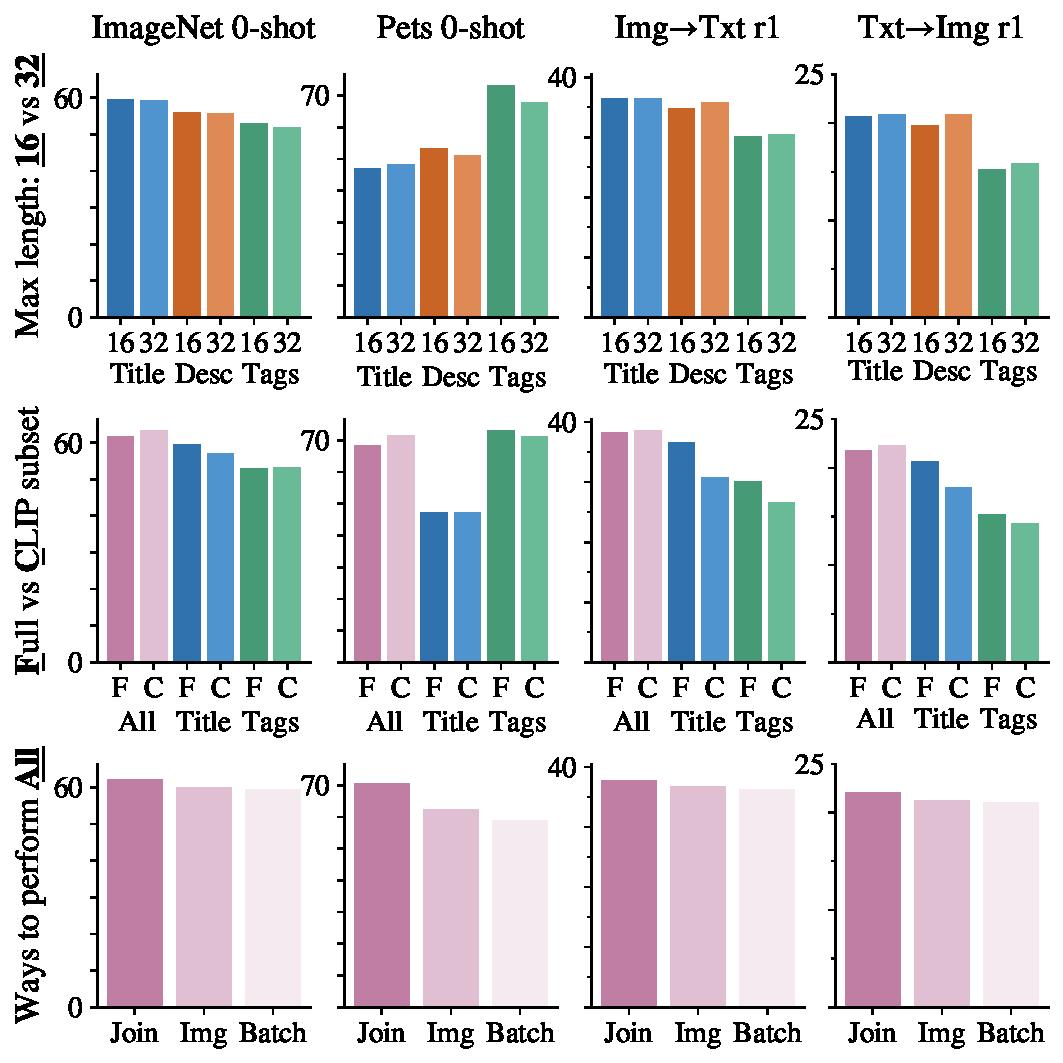
\includegraphics[width=\linewidth]{images/yfcc_choices.pdf}
    \caption{Ablations for YFCC100m.
    \textbf{Top:} even though the description field can be long, the potential benefit of using more than 16 tokens does not outweigh the increased memory and computation cost.
    \textbf{Middle:} When using all text signals, sticking to the CLIP subset is better according to the standard benchmarks, however see also Section~\ref{sec:multilingual}.
    \textbf{Bottom:} Using all three text signals simultaneously for all examples works better than sampling one per image or per batch.}
    \label{fig:yfcc}
\end{figure}

The YFCC100m dataset comes with a rich set of annotations for each image, including camera settings and geolocation.
Out of all the annotations, three of them are potential candidates for learning image-text pairings: the image's title, a description, and a set of free-form tags.
However, only partially overlapping subsets of 60\,M, 30\,M, and 65\,M images come with a title, description, or tags, respectively.
We first explore which supervision signal is most useful.
For the description, we simply tokenize the provided text; for the title, we perform basic filtering and remove titles that start with {\tt DSC}, {\tt IMG}, {\tt Picture}, consist of only the word {\tt image} or consist of more than half digits; for the tags, we randomly shuffle their order, and join them with a random space, newline, or basic punctuation character in order to get a string which we then tokenize.
The texts vary dramatically in length, we thus try maximum sequence lengths of 16 and 32 tokens.
The first row of Figure~\ref{fig:yfcc} shows the result of this experiment.
The difference between a maximum sequence length of 16 and 32 is small, however the memory savings are substantial and we thus restrict the sequence length to 16 tokens in all further experiments.

In terms of supervision signal, there is no single clear winner. We thus explore three ways of learning from all signals and so also make use of the full 100\,M images. We can either \emph{join}tly optimize them by summing up three contrastive losses for each image, or we can randomly sample one of the three sources for each \emph{image} or for a whole mini\emph{batch}. As can be seen in the bottom row of Figure~\ref{fig:yfcc}, jointly using all signals consistently works better, although it requires triple the amount of passes through the text tower.

Finally, the authors of CLIP~\cite{clip} provide a curated subset of roughly 15\,M images, which contain high quality annotations in English. We refer to this subset as YFCC\textsubscript{CLIP}.
In the middle row of Figure~\ref{fig:yfcc}, we compare how using the \emph{F}ull YFCC100m for \lit compares to using the \emph{C}LIP subset of it. Both seem to perform roughly on par for all signals for classification, but when using only titles or tags and performing image-text retrieval, it is better to apply \lit on the full YFCC100m dataset.

Overall, we obtain the best results with \lit using all text signals jointly on the YFCC\textsubscript{CLIP} subset. However, this investigation was performed with the small ViT-B/32 model, it is likely that a larger model may perform better when using the full dataset.


\section{Effective batch size for contrastive loss}
\label{appendix:batch_size}

\begin{figure}[t]
    \centering
    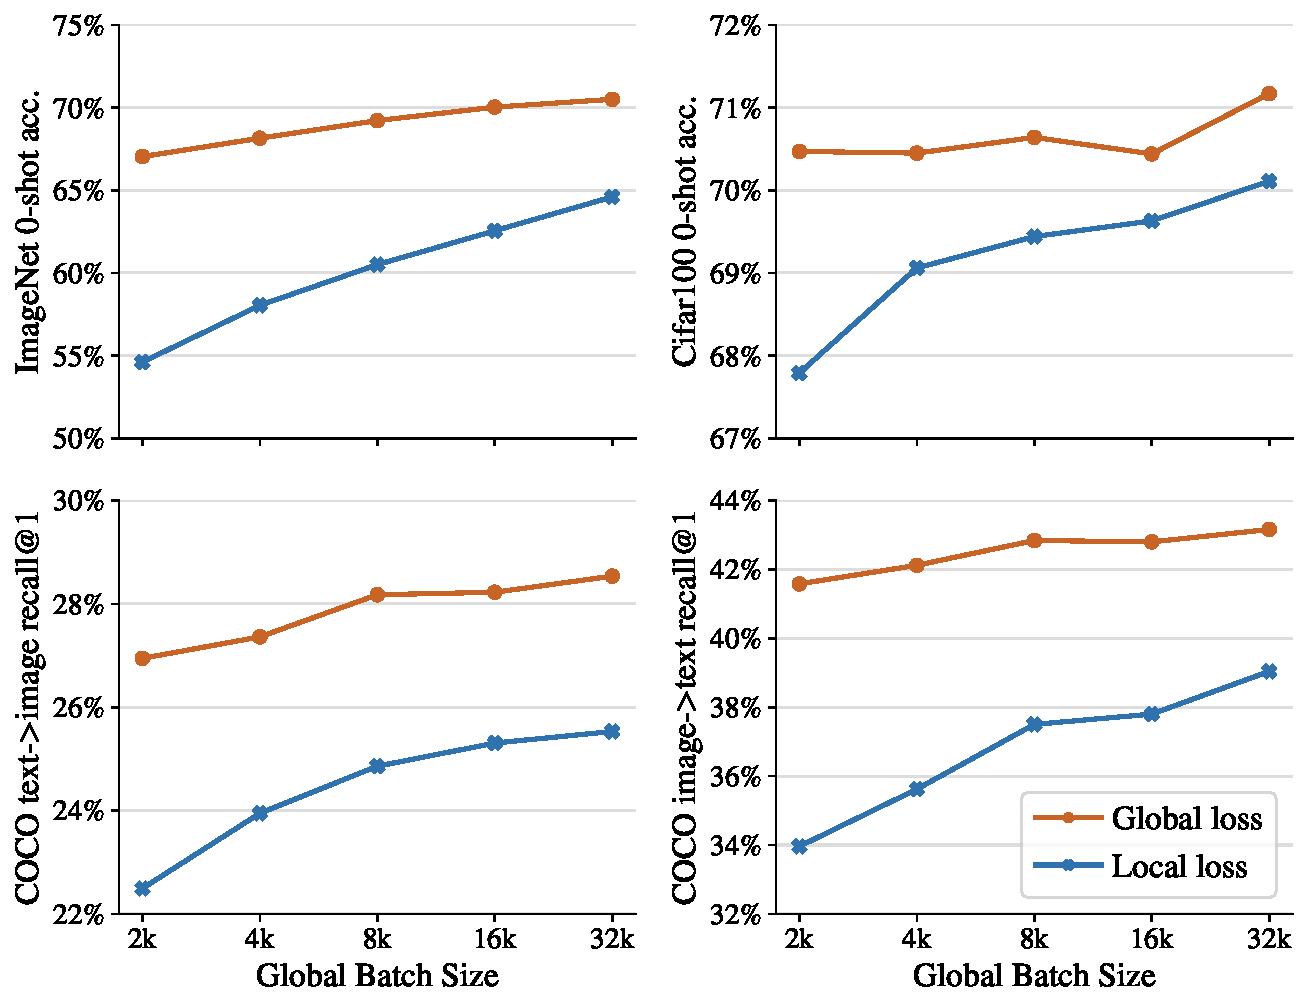
\includegraphics[width=\columnwidth]{images/batch_size.pdf}
    \caption{Impact of batch sizes for contrastive loss, including both global contrastive loss and local contrastive loss.}
    \label{fig:batch_size}
\end{figure}

In this section, we study the impact of the effective batch size for contrastive loss.
We use the \Lu setup with a pre-trained B/32 image model, tuned for 900 million seen image-text pairs.
In Figure~\ref{fig:batch_size}, we see a clear improvement when using global contrastive loss.
It has increased the effective batch size for contrastive learning, thus introducing more hard negatives and improving model quality.
Interestingly, we found that larger batch size leads to better performance consistently.
We leave extremely large batch size exploration to future work.

% ===============================================
% ===============================================

\section{Pre-computation for locked image models}
\label{appendix:precompute}

In \lit{} method, the locked image model generates identical embeddings given the same image. 
Based on this characteristic, we use pre-computed image embeddings during tuning.
It allows faster iterations and fitting larger text models in memory, as the image representations are extracted only once and no image models are loaded. 

\begin{figure}[t]
    \centering
    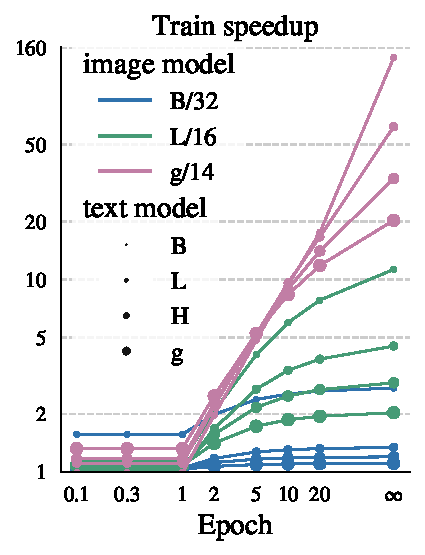
\includegraphics[width=0.236\textwidth]{images/precompute_epoch.pdf}
    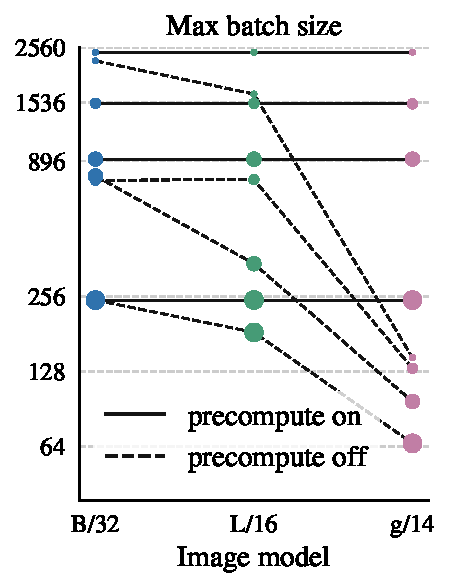
\includegraphics[width=0.236\textwidth]{images/precompute_maxbatch.pdf}
    \caption{\textbf{Left}: Pre-computing image embeddings accelerates \lit{}, when tuning for more than a single epoch. 
    \textbf{Right}: Pre-computing image embeddings in \lit{} allows larger batch size in memory.}
    \label{fig:precompute}
\end{figure}

Figure~\ref{fig:precompute} left shows how training speeds up as the number of epochs grows.
When training no more than a single epoch, pre-computation keeps a constant speed ratio over re-computation, which increases from one (same speed) to larger than one (speedup) as image model size grows.
After one epoch, pre-computation clearly accelerates training due to reused image representations. 
The speedup ratio becomes more visible as either the number of epochs or the image model size grows.

For experiments with pre-computed image embeddings, we count both pre-computation inference cost and tuning cost. 
Pre-computation will be performed on at most a single epoch on the image-text dataset.
In practice, the pre-computed embeddings can be shared across different experiments, as long as the image tower is identical. 
As a result, the actual cost is even lower than our estimation.
For experiments without pre-computed image embeddings, we count the actual contrastive-tuning cost.

Pre-computation eliminates loading the image model to memory during training, thus allowing larger batch sizes for contrastive loss. 
We search maximum batch sizes on each combination of image and text models with and without pre-computation, and show the results in Figure~\ref{fig:precompute} right. We search for the maximum batch size for each model with a unified setup. We report the maximum batch size that the model can fit on 8 TPU v3 cores.

However, if image augmentations are enabled during training, we may not benefit much from pre-computation.
The model sees different augmented images in multiple epochs.
Nevertheless, the memory benefits still hold.
All metric details are in Table~\ref{tab:precompute_details}.

\begin{table}
\centering
\small
\setlength{\aboverulesep}{0pt}
\setlength{\belowrulesep}{0pt}
\begin{tabular}{l@{\hspace{5pt}}l|r@{\hspace{5pt}}r|r@{\hspace{5pt}}r@{\hspace{5pt}}r|r@{\hspace{5pt}}r}
\toprule
\multicolumn{2}{c|}{}&\multicolumn{2}{c|}{}&\multicolumn{3}{c|}{}&\multicolumn{2}{c}{}\\[-6pt]  % vertical padding
\multicolumn{2}{c|}{\bf{Model}}&\multicolumn{2}{c|}{\bf{Param (M)}}&\multicolumn{3}{c|}{\bf{Max speed}}&\multicolumn{2}{c}{\bf{Max batch}}\\[1.5pt]
\arrayrulecolor{lightgray}\midrule[0.25pt]\arrayrulecolor{black}
Image&Text&Pre&Non&Pre&Non&Inf&Pre&Non\\
\hline
B/32&B&105&195&2439&893&3294&2448&2262\\
B/32&L&320&410&924&688&3294&1528&751\\
B/32&H&640&730&468&390&3294&912&781\\
B/32&g&1007&1097&242&218&3294&248&248\\
L/16&B&105&406&2423&215&273&2448&1663\\
L/16&L&320&621&920&204&273&1528&754\\
L/16&H&640&942&465&160&273&912&347\\
L/16&g&1007&1308&240&118&273&248&184\\
g/14&B&105&1094&2409&17&17&2448&146\\
g/14&L&320&1310&932&15&17&1520&132\\
g/14&H&641&1630&467&14&17&912&97\\
g/14&g&1008&1997&243&12&17&248&66\\
\bottomrule
\end{tabular}
\caption{Pre-computation details. \emph{Max speed} and \emph{Max batch} describe metrics collected by maximum speed (img/sec/core) and batch size, respectively, corresponding to Figure~\ref{fig:precompute}. \emph{Pre} and \emph{Non} are metrics with and without pre-computation respectively; \emph{Inf} describes pre-computation inference speed, which is only affected by image models. All experiments are run on 8 TPU v3 cores.}
\label{tab:precompute_details}
\end{table}

\section{Learning rate schedules}
\label{appendix:lr_schedules}

\begin{figure}[t]
    \centering
    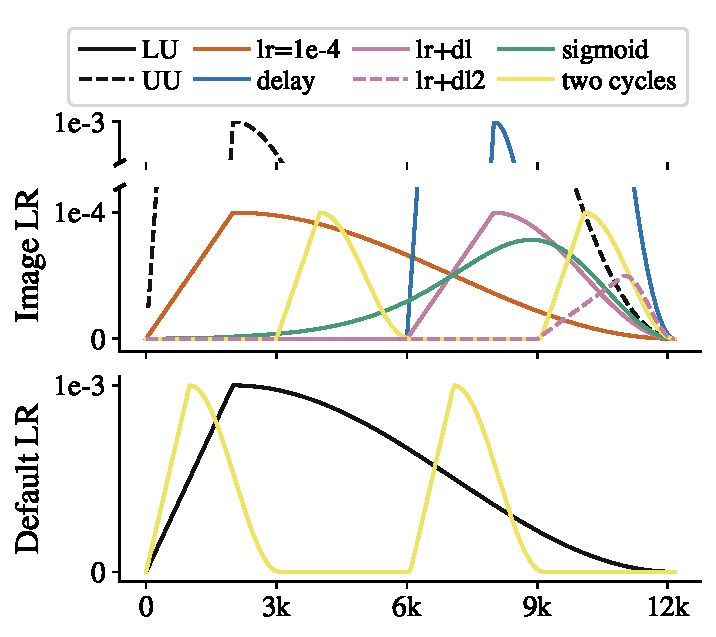
\includegraphics[width=.35\textwidth]{images/lr_schedules.pdf}
    \caption{Different learning rate schedules. Note that the default LR schedule is shown in black in the lower part of the figure.}
    \label{fig:lr_schedules}
\end{figure}

\begin{figure}[t]
    \centering
    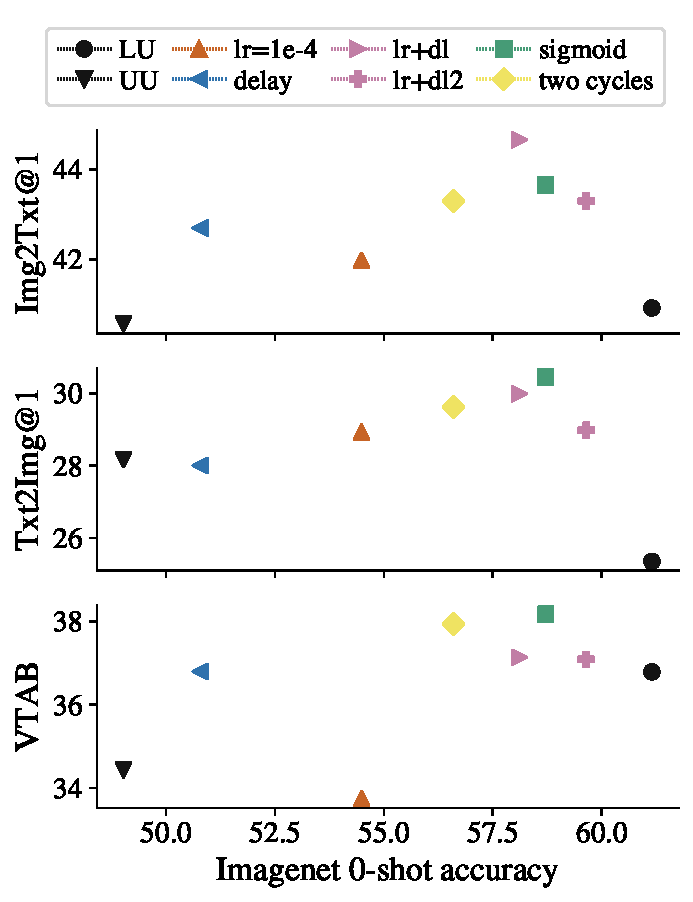
\includegraphics[width=.35\textwidth]{images/lr_pointcloud.pdf}
    \caption{ITR and VTAB metrics as a function of ImageNet 0-shot accuracy for different LR schedules.}
    \label{fig:lr_pointcloud}
\end{figure}

For most of the experiments, weights were either completely locked, or trained with the same learning rate schedule (linear warmup and cosine decay). We experimented with different learning rate schedules (Figure~\ref{fig:lr_schedules}), mainly varying how the image tower was updated. We observed that training the image tower with a smaller learning rate and/or delaying training of the image tower resulted in better retrieval metrics (Figure~\ref{fig:lr_pointcloud}).

The default schedules (LU and UU) have the best and worst ImageNet 0-shot accuracy of all tried learning rate schedules. Compared to UU, both ITR/VTAB metrics and ImageNet 0-shot accuracy improve modestly, when the image learning rate is only scheduled for the second half of the training (“delay"). The ImageNet 0-shot accuracy improves more but the VTAB accuracy drops when the learning rate is set to a smaller value (“lr=1e-4"). Combining the delay with the smaller learning rate (“lr+dl") further improves both ITR/VTAB metrics and ImageNet 0-shot accuracy. A similar result is achieved by multiplying the learning rate in the UU setting with a sigmoid function (“sigmoid"). Alternating between freezing image tower and rext tower (“two cycles") finally performs somewhere between “lr+dl" and “lr=1e-4" schedules.

\section{Zero-shot transfer details}
\label{appendix:zero-shot-details}
\subsection{Classification}

We follow CLIP~\cite{clip} for the zero-shot transfer evaluation. We use the identical ImageNet class label names and the same 80 prompt templates as in CLIP.
During evaluation of private LiT models, we first resize the test image and then central crop with 0.875 aspect ratio to the target resolution. More specifically, we use $224\times224$ target resolution for CIFAR dataset and $288\times288$ target resolution for the remaining datasets.
For all the public LiT models, we resize all test images to $224\times224$ for simplicity.


\subsection{VTAB Evaluation}
\label{appendix:vtab}
The Visual Task Adaptation benchmark\cite{vtab} consists of 19 diverse visual tasks. We refer readers to the original publication for details about each dataset; here we just mention that they are split into three categories:
\begin{itemize}
    \item \textbf{Natural}: These tasks contain classical “natural” real-world images obtained with a camera, such as vehicles, pets, scenery and household objects.
    \item \textbf{Specialized}: These are datasets of arguably “natural” images which were captured with specialised photographic equipment, such as satellite photographs and medical images.
    \item \textbf{Structured}: These assess understanding of scenes structure in some way, predominately from synthetic environments. Example tasks include 3D depth estimation and counting.
\end{itemize}
Note that there is significant overlap with the datasets assessed in~\cite{clip}, but it is not guaranteed that the same data splits were used.

\textbf{Evaluation protocol.} 
Previous works\cite{clip} define task-specific prompts and class names, but it is not clear exactly how an optimal set of prompts for a given task was chosen.

For VTAB, we define a search space of image preprocessing, prompt templates and classes, where the latter two are often per-task (e.g. using `a` `satellite` `photo` `of` `...` or `an` `overhead` `photo` `of` `...` for tasks involving satellite imagery). All such settings are tried on a small validation set of 800 images, and the optimal setting is then run on the official VTAB test set.

We note this is arguably not \textit{zero-shot} transfer, but believe it is a principled and reproducible approach.

\textbf{Prompts used.}
For all tasks, we considered 3 default sets of prompts
\begin{enumerate}
\item \texttt{A photo of a \cls}
\item \texttt{\cls}
\item The 6 CLIP prompts used for ImageNet\footnote{https://github.com/openai/CLIP/blob/main/data/prompts.md}
\end{enumerate}

We also consider some task specific prompts/class name settings. Note that these two degrees of freedom are orthogonal, and a text setting is defined by both. They are shown in  Table~\ref{tab:vtab_prompts_default} and Table~\ref{tab:vtab_prompts_custom}. Not all of these prompts were equally useful; some are redundant, providing equal performance gain as other settings, and some do not provide performance gains at all. We show the performance delta comparing only the default prompts versus including a given text variant as well, to give a rough idea of how beneficial it was.


\textbf{Can we assess zero-shot performance using VTAB?}
The strength of such a diverse benchmark is in the variety of its label spaces. ImageNet classes, though very fine-grained, are fairly generic. However, VTAB also includes \textit{structured tasks} which are designed to assess the model's competence at tasks which aren't object recognition, such as counting and assessing distances and angles.
This presents interesting difficulties for solving in a zero-shot natural language grounded manner. Figure \ref{fig:vtab_cat} shows the zero-shot performance of many models developed for this paper. Their detailed performance is not important here - the gray lines show what a “random guesser” would achieve on each VTAB category. It is not an obvious number, as performance across categories is an average of all the constituent datasets, which have varying numbers of classes.
It is clear from this figure that the structured performance does not significantly deviate from random guessing, despite extensive efforts in prompt engineering. We leave it as an open - and very interesting - research direction to figure how to make such models count and assess distances. Furthermore, though contrastive image-text training on the web can largely match supervised models on natural tasks, further improvements are needed on more specialist tasks.

\begin{figure}[t]
    \centering
    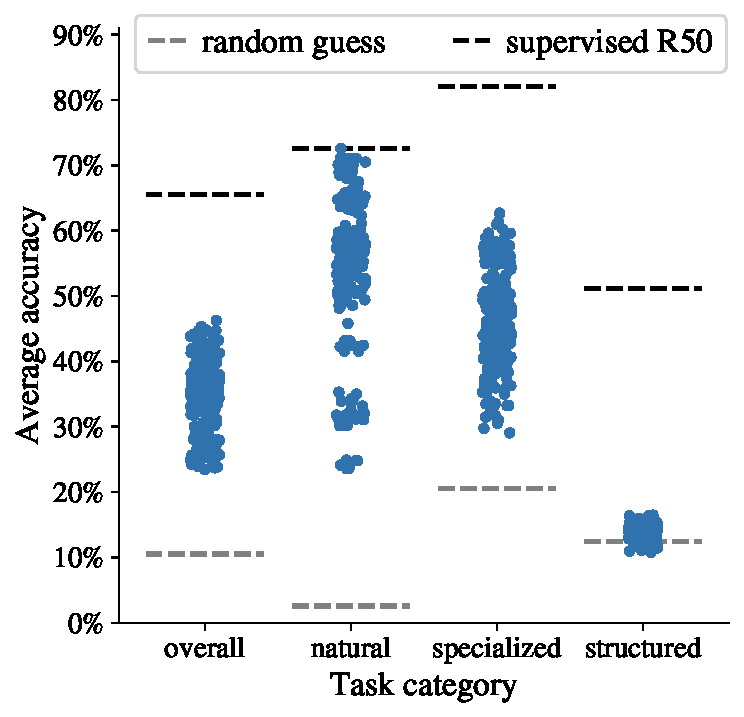
\includegraphics[width=.7\linewidth]{images/vtab_categories.pdf}
    \caption{Performance of zero-shot classification models across different VTAB categories. Each dot is a zero-shot model evaluation.}
    \label{fig:vtab_cat}
\end{figure}

\subsection{Cross-modal retrieval}

We compute retrieval metrics on MSCOCO captions~\cite{mscoco}, reporting the numbers on the test set (5\,000 images, 25\,010 captions).
%
For the image to text retrieval, we rank all texts by decreasing cosine similarity of their embedding with the image embedding, and then report the fraction of images that ranks the correct text within the first (1, 5, 10) positions as the Recall@1, Recall@5, Recall@10 metrics.
For the text to image retrieval, we compute the same metric, but ranking images and averaging over all texts.
When showing a single number, we always refer to the Recall@1 metric.


\section{Multilingual details and limitations}
\label{appendix:multilingual_details}

\begin{figure*}[t]
    \centering
    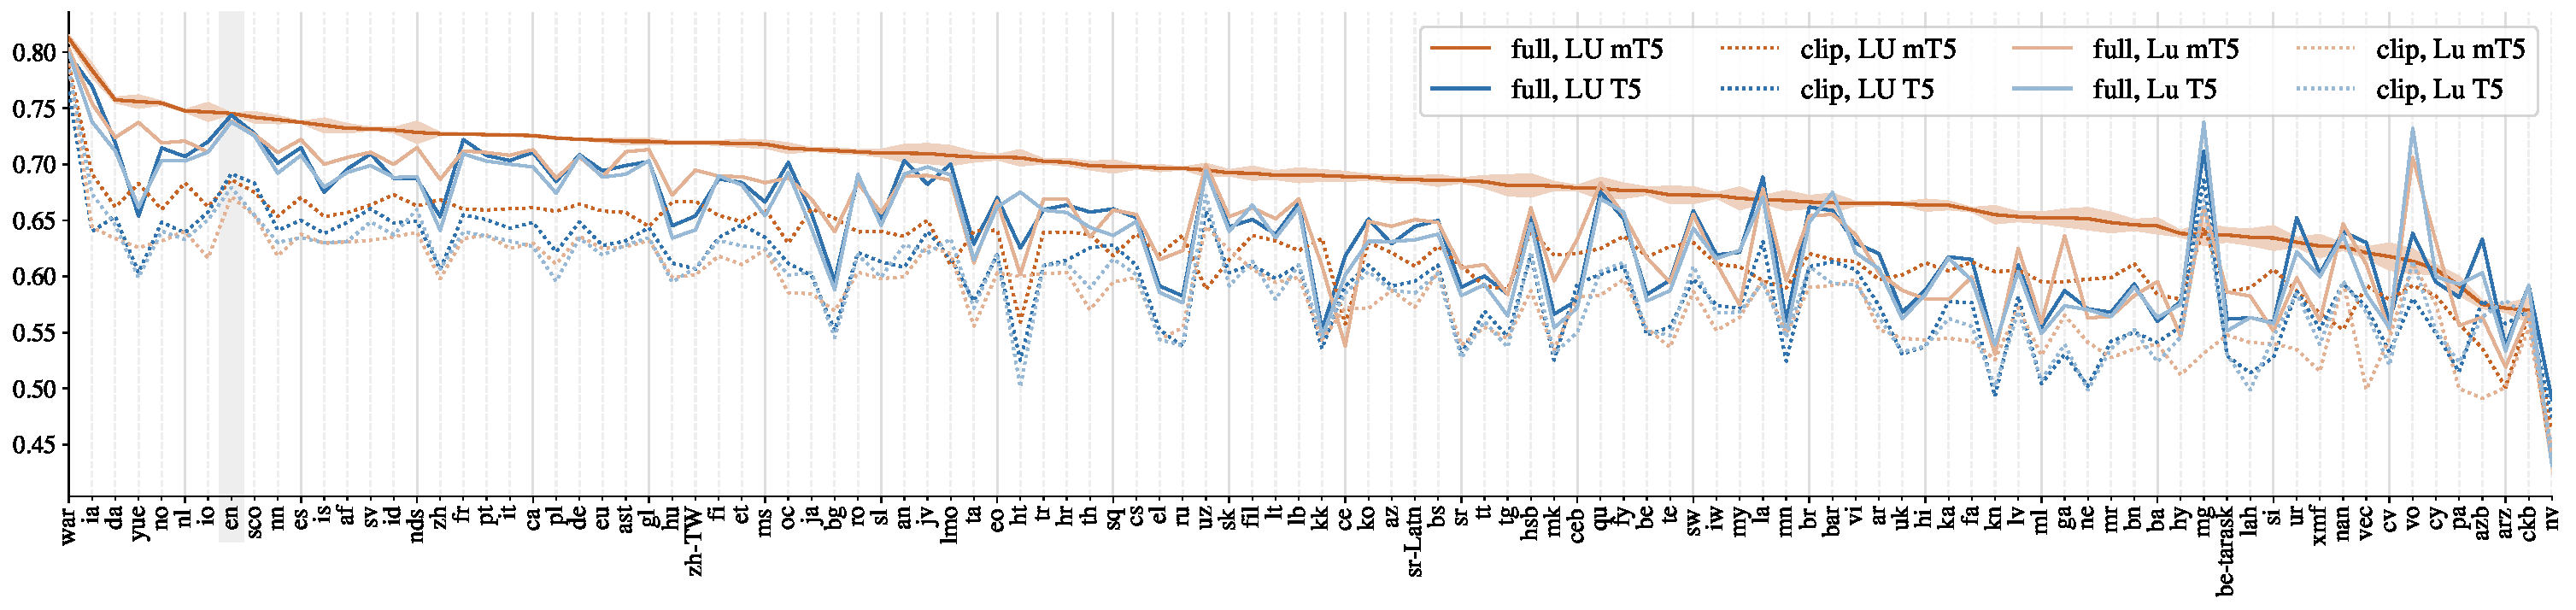
\includegraphics[width=\textwidth]{images/xlang_wit_wide.pdf}
    \caption{Fully detailed evaluation of the multilingual models on WIT.}
    \label{fig:xlang_wit_wide}
\end{figure*}

\textbf{Extra results.}
Table \ref{tab:yfcc_xlang} shows the English zero-shot ImageNet classification performance of different English and multilingual T5 models, with \lit{} on YFCC\textsubscript{CLIP} vs. YFCC100m. We note that training on the larger, more diverse, multilingual set does not come at the expense of English performance.
\begin{table}
\centering
\begin{tabular}{>{\kern-\tabcolsep}lcccccc<{\kern-\tabcolsep}}
\toprule
 & \multicolumn{3}{c}{CLIP subset} & \multicolumn{3}{c}{Full} \\
{} &    \textbf{ImgNet} &   \textbf{T$\rightarrow$I} &   \textbf{I$\rightarrow$T} & \textbf{ImgNet} &   \textbf{T$\rightarrow$I} &   \textbf{I$\rightarrow$T} \\
\midrule
T5 &        58.9 &  14.5 &  22.6 &     62.4 &  19.6 &  34.3 \\
\rowcolor{gray!20} 
\textit{ + pt} &        58.5 &  17.2 &  29.1 &     62.3 &  \textbf{20.1} &  \textbf{34.5} \\
mT5       &        58.7 &  14.4 &  23.1 &     62.1 &  18.5 &  32.6 \\
\rowcolor{gray!20}
\textit{ + pt} &        58.4 &  15.6 &  25.1 &     \textbf{62.6} &  18.9 &  33.6 \\
\bottomrule\end{tabular}
\caption{Training on the full YFCC100m data significantly improves all metrics compared to the CLIP subset. Gray rows are with text pre-training.}
\label{tab:yfcc_xlang}
\end{table}

\textbf{Wiki-Image Text as an evaluation benchmark.} We noted qualitatively that, as one may expect from Wikipedia, a large proportion of examples are about entities such as people, places, or art. When translated to other languages, proper nouns are usually kept as is - especially if the two languages share an alphabet. This makes it an imperfect dataset to benchmark multilinguism as monolingual models will score higher than they should.

\textbf{Tokenization subtleties.} The sentencepiece tokenizers, when faced with unknown vocabulary, will default to byte encoding. This is not a perfect catch-all; in such circumstances models cannot take advantage of pre-training, and the resultantly very long sequences will not fit in the 16-token maximum length used in this paper. It is nevertheless better than the `[UNK]` tokens produced by BERT's WordPiece tokenizer; with SentencePiece, even with an imperfect vocabulary, the model has a chance to adapt. This explains why even with an ill-suited English-only vocabulary, the T5 models can still learn decent representations of non-English languages.

\textbf{Translation of prompts.} One obvious factor worth noting is that, in our setup, non-English languages may be impacted by imperfect translations. This likely means non-English performance is underestimated.

More subtly, we note that many languages - especially those with Latin alphabets - often use the English word for very niche or specific items. For example, at the time of writing, the Vietnamese translation of `I` `took` `a` `photo` `of` `an` `airship` contains the word `airship` verbatim. The contrastive model can in principle pick out the word `airship`, ignore all the Vietnamese, and retain decent performance despite not understanding Vietnamese at all.

\textbf{Backtranslation as data augmentation.}
Backtranslation\cite{backtranslate} - translating to a language and back again, in order to generate slightly different versions of a given text - is a common augmentation in NLP. We run some experiments to see whether it works for contrastive image-text training.
We again use an online translation service to translate the texts in CC12M to and from 9 different languages. This probability is shared across the languages i.e. a backtranslation probability of 0.5 with 5 different backtranslate candidates means there is a 50\% chance of picking the original ground truth and a 10\% chance each of picking one of the backtranslated candidates.
Figure \ref{fig:backtranslate} shows the effect of this augmentation on \lit{} using an AugReg ImageNet21k pre-trained ViT-B/16 model. Backtranslation is fairly useful up to certain point, with 10\% giving a good trade-off which improves all metrics.

\begin{figure}[t]
    \centering
    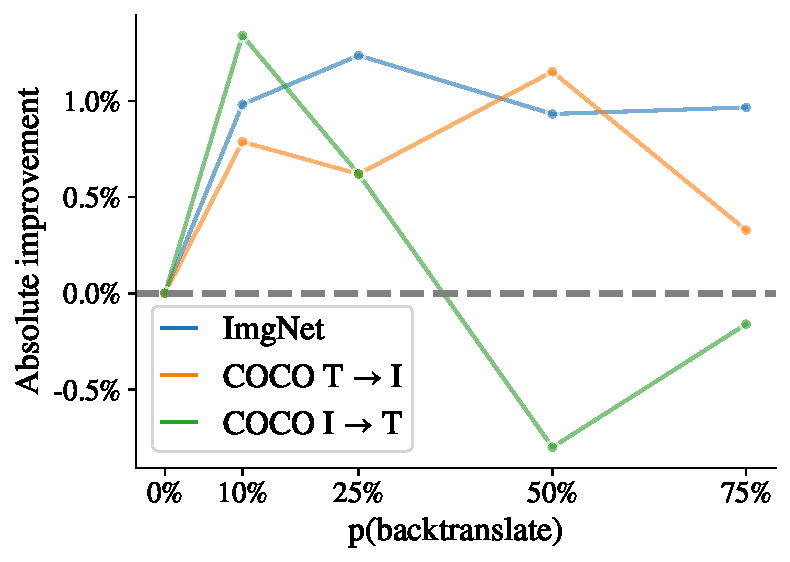
\includegraphics[width=.8\linewidth]{images/backtranslate.pdf}
    \caption{Backtranslating data as a form of data augmentation improves performance across most metrics.}
    \label{fig:backtranslate}
\end{figure}

\section{More de-duplication results}
\label{appendix:more_dedup}

We present more ablation test results using larger architectures. 
We aim to check whether larger architectures be\-ne\-fit more from duplicates, while small architectures do not have enough capacity to overfit to the duplications.
More specifically, we adopt the \Lu setup with a pre-trained ViT-L/16 image model~\cite{vitg}, and from-scratch L size text model.
Table~\ref{table:duplicates_l16} shows the experimental results. We find that the conclusions are consistent with the runs using the ViT-B/32 image model discussed in Section~\ref{sec:deduplication}. 
This is further evidence suggesting that duplications are not the root cause for good zero-shot transfer results.

\begin{table}[t]
  % \small
  \newcolumntype{C}{>{\centering\arraybackslash}X}
  \newcolumntype{R}{>{\raggedleft\arraybackslash}X}
  \setlength{\tabcolsep}{0pt}
  \setlength{\extrarowheight}{5pt}
  \renewcommand{\arraystretch}{0.75}
  \centering
  % Format is type{width}, p: paragraph, top-align, C is custom, c is squeezed.
  \begin{tabularx}{\linewidth}{p{1.5cm}p{0.1cm}Cp{0.1cm}Cp{0.1cm}Cp{0.1cm}Cp{0.1cm}C}
    \toprule[1pt]
     \bf{Dedup} && \bf{\# up.} && \bf{\# down.} && \bf{ImgNet} && \bf{I$\rightarrow$T} && \bf{T$\rightarrow$I}\\
    \midrule
     - && 0 && 0 && 80.2 && 50.4 && 34.6 \\
     test && 2.6M && 76K && 80.2 && 49.0 && 34.3 \\  % 2_575_200
     train+test && 3.6M && 220K && 80.0 && 49.6 && 34.6 \\  % 3_637_630
    \bottomrule[1pt]
  \end{tabularx}
  \caption{Results on three different de-duplication setups, Lu setup with pre-trained ViT-L/16 image model.}\label{table:duplicates_l16}
\end{table}

\section{Image-text dataset comparison}
\label{appendix:align_vs_our}

\begin{table}[t]
  % \small
  \newcolumntype{C}{>{\centering\arraybackslash}X}
  \newcolumntype{R}{>{\raggedleft\arraybackslash}X}
  \setlength{\tabcolsep}{0pt}
  \setlength{\extrarowheight}{5pt}
  \renewcommand{\arraystretch}{0.75}
  \centering
  % Format is type{width}, p: paragraph, top-align, C is custom, c is squeezed.
  \begin{tabularx}{\linewidth}{p{1.5cm}p{0.1cm}Cp{0.1cm}Cp{0.1cm}Cp{0.1cm}C@{\hspace{-1ex}}}
    \toprule[1pt]
     \bf{Task} && \bf{Pairs Seen} && \bf{our} && \bf{ALIGN} && \bf{Diff.}\\
    \midrule
     ImageNet && 900M && 70.1 && 69.8 && 0.3\\
     ImageNet && 3.6B && 72.0 && 71.5 && 0.5\\
     ImageNet && 7.2B && 72.4 && 71.8 && 0.6\\
     ImageNet && 18B && 72.9 && 72.2 && 0.7\\
    \bottomrule[1pt]
  \end{tabularx}
  \caption{Comparing the ALIGN data with our data, which uses simpler text filters. }\label{table:align_vs_our}
\end{table}

Using simpler text filters for our dataset leads to a larger dataset size compared to the ALIGN dataset:
The ALIGN dataset contains 1.8B image-text pairs, while our data set contains 3.6B image-text pairs. 

In table~\ref{table:align_vs_our}, we show the results from training a baseline ViT-B/32 model on both datasets, with the same schedules. 
We vary the training schedule from 900M seen images, to 18B seen images.
We use 18B images to make sure that the training process is long enough to benefit from a larger dataset.
We find that the difference between the two datasets are small when the model is trained for a short period, \ie less than a single epoch.
As the training becomes longer, the impact of the dataset size becomes more visible.

Overall, the above results indicate that larger dataset with simpler filters slightly outperforms a smaller dataset with more filters.
We leave the thorough exploration of this topic to future work.


\begin{figure*}[t]
    \small
    \centering
    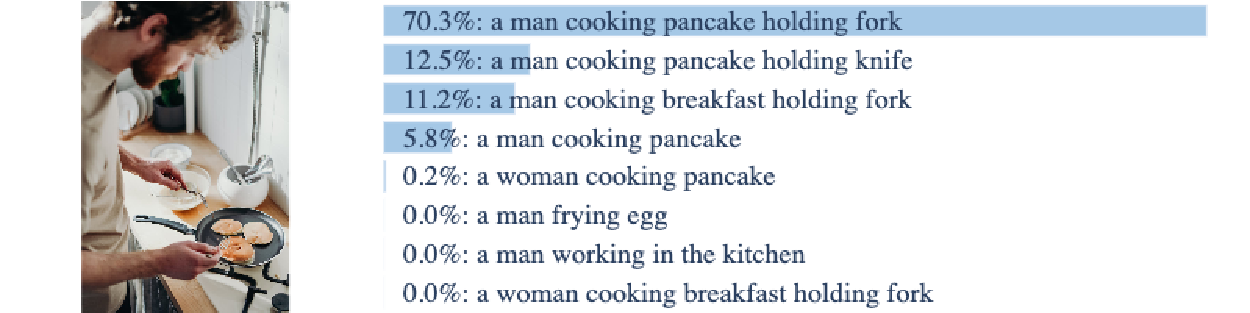
\includegraphics[width=0.495\textwidth]{images/demos_pdf/man_cooking_plot.pdf}
    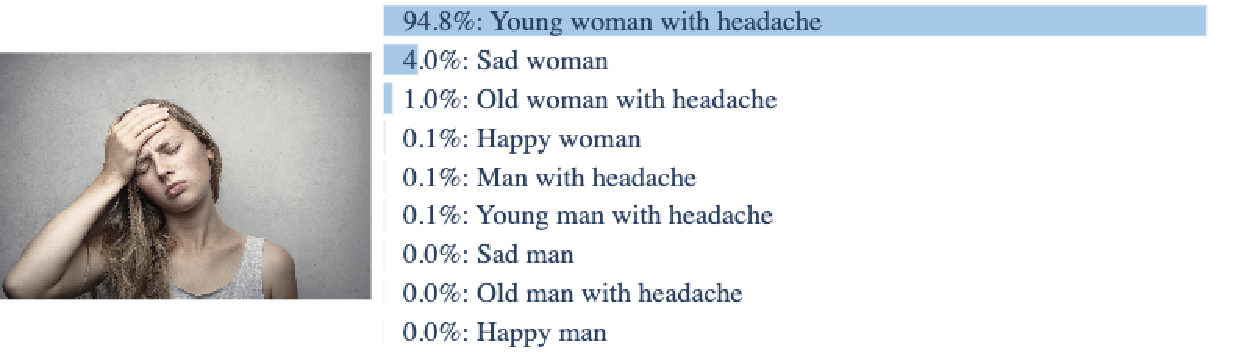
\includegraphics[width=0.495\textwidth]{images/demos_pdf/woman_headache_plot.pdf}
    \textbf{(a) Nuanced context}: The model can understand information such as actions or implied symptoms.
    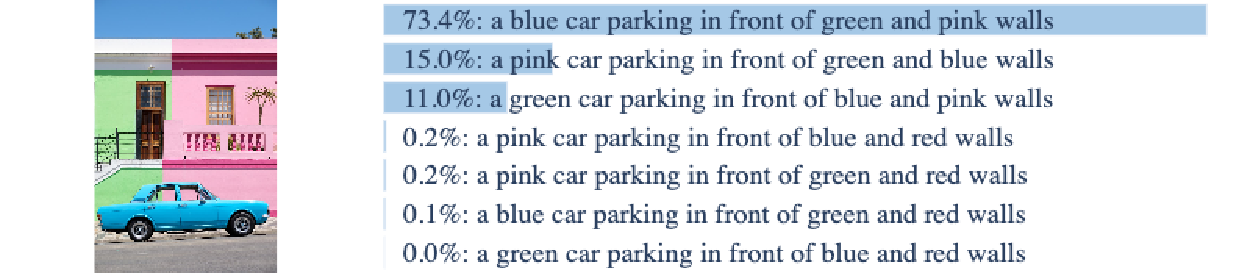
\includegraphics[width=0.46\textwidth]{images/demos_pdf/color_cars_plot.pdf}
    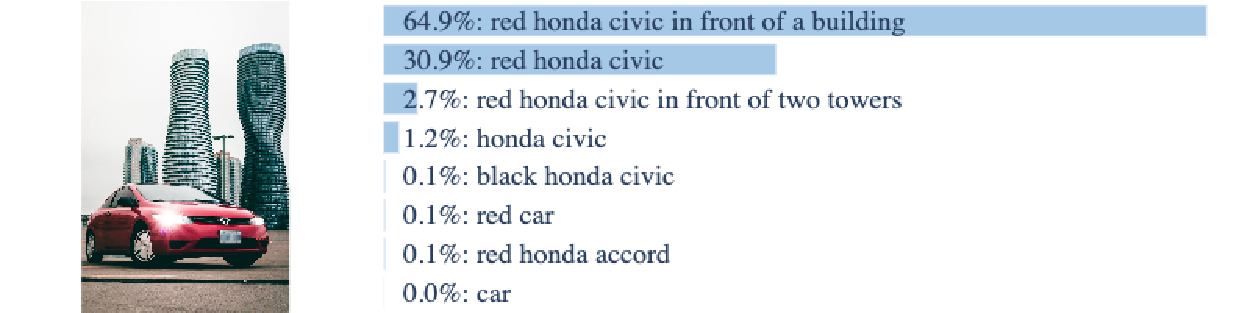
\includegraphics[width=0.53\textwidth]{images/demos_pdf/car_towers_plot.pdf}
    \textbf{(b) Richer information}: The model correctly handles colours, background buildings and even car brands.
    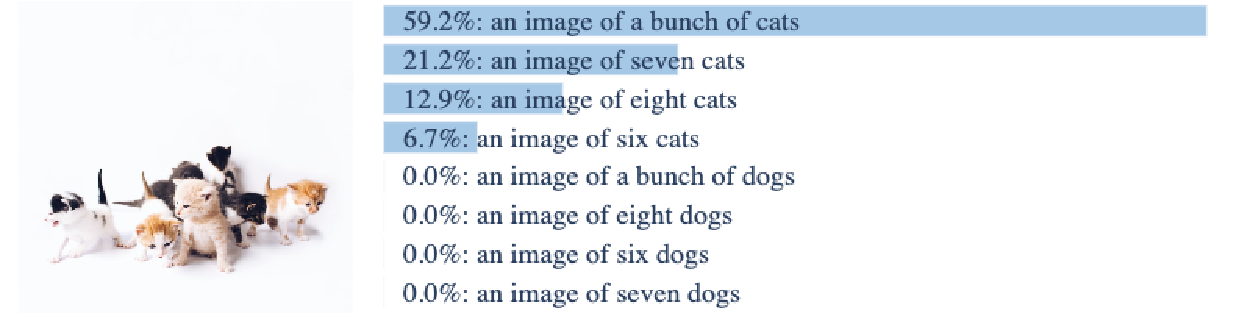
\includegraphics[width=0.495\textwidth]{images/demos_pdf/kitten_words_plot.pdf}
    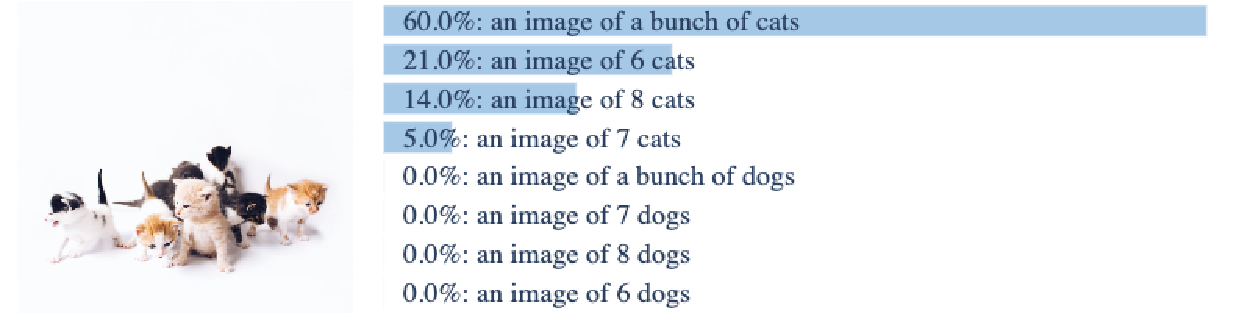
\includegraphics[width=0.495\textwidth]{images/demos_pdf/kitten_plot.pdf}
    \textbf{(c) Counting}: The model does a reasonable job at counting, though prompts like “bunch of cats" are preferred.
    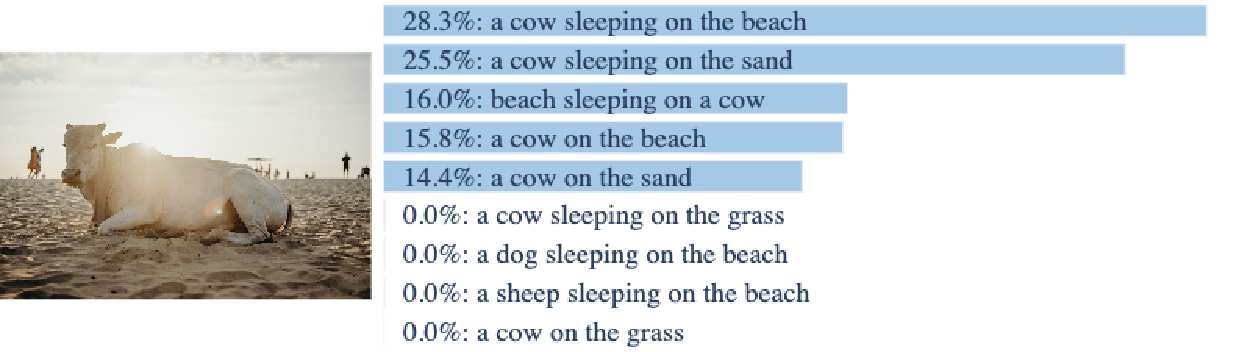
\includegraphics[width=0.495\textwidth]{images/demos_pdf/cow_beach_plot.pdf}
    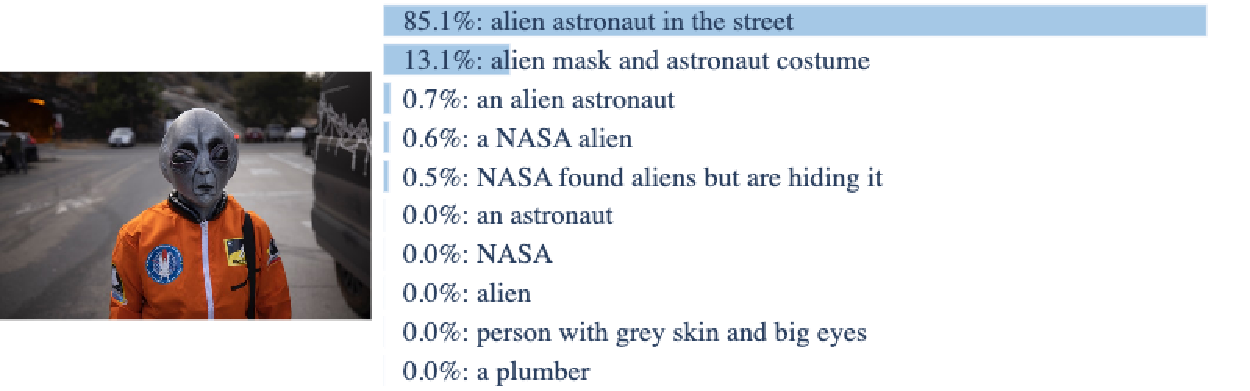
\includegraphics[width=0.495\textwidth]{images/demos_pdf/astronaut_alien_plot.pdf}
    \textbf{(d) Esoteric examples}: The model has no problems at identifying rare concepts, like a cow on a beach, or an astronaut alien.
    \caption{Various model predictions.}
    \label{fig:success_examples}
\end{figure*}

\begin{figure*}[h]
    \small
    \centering
    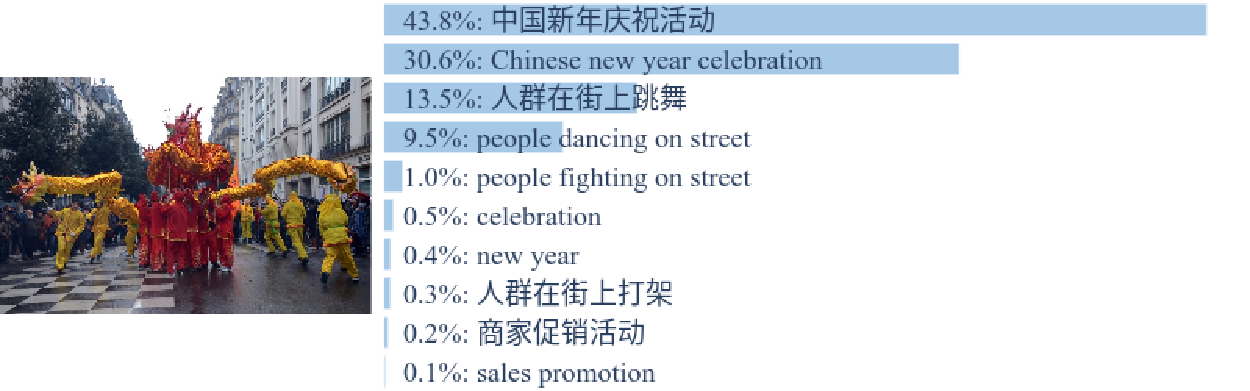
\includegraphics[width=0.495\textwidth]{images/demos_pdf/cny.pdf}
    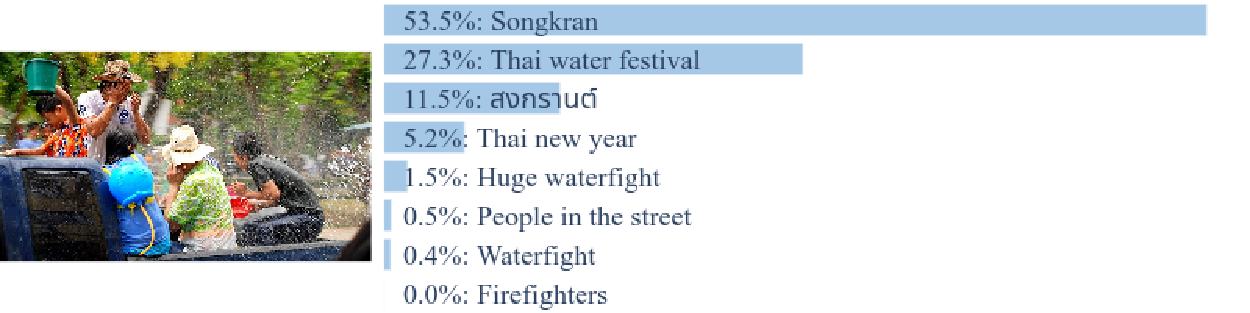
\includegraphics[width=0.495\textwidth]{images/demos_pdf/songkran.pdf}
    \caption{Training on multilingual data allows the model to recognise concepts in multiple languages, including visual concepts which do not directly exist in English.}
    \label{fig:xlang_examples}
\end{figure*}

\begin{figure*}[h]
    \small
    \centering
    
\includegraphics[width=0.45\textwidth]{images/demos_pdf/emoji_yawn_fig1.pdf}
    
\includegraphics[width=0.54\textwidth]{images/demos_pdf/emoji_yawn_fig2.pdf}
    \textbf{}
    \caption{Qualitative failures. In the left example, the model ranks the wrong grinning face before the ground truth yawning face. However, by removing the grinning face and adding emoji prompt, the model prefers emoji yawn.}
    \label{fig:failure_examples}
\end{figure*}

\section{Qualitative examples}
\label{appendix:demos}
Though strong classification \& retrieval performance is promising, it arguably probes understanding of very simple concepts. Are \lit{} models really zero-shot learners capable of understanding open vocabularies?

We touch here on a few qualities these models should ideally have, but note that these are not to be considered representative; benchmarks that investigate more than simply fine grained visual classification should be used to more thoroughly understand these phenomena.

\subsection{Private LiT model}
In this section, we present model predictions with manually constructed image-text pairs input. Results from private LiT model are shown in Figure~\ref{fig:success_examples}. We believe that with LiT, we successfully made a pre-trained image model to a zero-shot learner, that supports classification and retrieval with open vocabularies instead of a fixed label set. 


\subsection{Multi-lingual model}
Thanks to LiT on the multilingual dataset, the model also supports inputs using different languages. In Figure~\ref{fig:xlang_examples}, we show results both in Thai and Chinese. The model recognized the “Songkran" event in Thai, and the “Chinese Spring Festival" event in Chinese; it nonetheless also ranks English translations or transliterations quite highly, which is likely reflective of the data distribution. 
Multilingual capability makes our models more inclusive and accessible to non-English speakers.


\subsection{Model failures}
We present model failures in Figure~\ref{fig:failure_examples}. We show examples of how one can slightly change the text candidastes to manipulate the model output; one can easily force a desired answer by tuning other text candidates to rank lower.


\input{vtab_table_default_classname.txt}

\newpage
\onecolumn
\input{vtab_table_custom_classname.txt}
\twocolumn


\begin{table*}
% \vspace{-1cm}
\centering
\label{table:main}
\footnotesize
\resizebox{\textwidth}{!}{%
\addtolength{\tabcolsep}{-1.7pt}% <- remove some horizontal white space between the columns for better text readability
\begin{tabular}{@{}llrlll@{\hspace{0.3ex}}llllrlrrrrrr@{}}
\toprule
                                      Ref & Dataset & Images &   Cfg &  H &        Image &        Text & Tok &     Inits & Optim &   LR &    WD & INet & T$\rightarrow$I & I$\rightarrow$T &   Vn &  Vsp &  Vst \\
\midrule
              Fig~\ref{fig:teaser_curve} &    YFCC\textsubscript{CLIP} &   983M &  \LU &  y &     vit-B/32 &   bert-base &  WP &   AR,Bert &  Adam & 8e-4 &  1e-4 & 63.6 &            22.1 &            37.6 & 59.3 & 35.0 & 12.7 \\
              Fig~\ref{fig:teaser_curve} &    YFCC\textsubscript{CLIP} &   983M &  \UU &  y &     vit-B/32 &   bert-base &  WP &   AR,Bert &  Adam & 3e-4 &  1e-5 & 53.3 &            23.4 &            37.6 & 54.9 & 44.4 & 14.1 \\
              Fig~\ref{fig:teaser_curve} &    YFCC\textsubscript{CLIP} &   983M &  \uu &  y &     vit-B/32 &   bert-base &  WP &       -,- &  Adam & 8e-4 &  1e-4 & 42.1 &            17.9 &            31.1 & 45.8 & 49.8 & 14.3 \\
    \arrayrulecolor{lightgray}\midrule[0.25pt]\arrayrulecolor{black}
                     Tab~\ref{table:sota} &    Ours &  18.2B &  \Lu &  n &    vit-g/14* &   vit-giant &  SP &     JFT,- &  Adaf & 1e-3 &     0 & 85.2 &            41.9 &            59.3 & 74.7 & - & - \\
                     Tab~\ref{table:sota} &   Mixed &   983M &  \LU &  y &     vit-L/16 &  bert-large &  WP &   AR,Bert &  Adaf & 8e-4 &  1e-4 & 75.7 &            31.2 &            48.5 & 63.1 & 50.3 & 14.1 \\
    \arrayrulecolor{lightgray}\midrule[0.25pt]\arrayrulecolor{black}
              Tab~\ref{table:design_our} &    Ours &   901M &  \Lu &  n &     vit-B/32 &    vit-base &  SP &     JFT,- &  Adaf & 1e-3 &     0 & 70.1 &            28.6 &            43.8 & 66.6 & 57.2 & 14.6 \\
              Tab~\ref{table:design_our} &    Ours &   901M &  \Uu &  y &     vit-B/32 &    vit-base &  SP &     JFT,- &  Adaf & 1e-3 &     0 & 57.2 &            27.0 &            40.1 & 60.1 & 58.0 & 15.0 \\
              Tab~\ref{table:design_our} &    Ours &   901M &  \uu &  y &     vit-B/32 &    vit-base &  SP &       -,- &  Adaf & 1e-3 &     0 & 50.6 &            24.1 &            38.9 & 55.3 & 38.9 & 16.5 \\
    \arrayrulecolor{lightgray}\midrule[0.25pt]\arrayrulecolor{black}
  Tab~\ref{table:more_image_pretrainings} &    YFCC\textsubscript{CLIP} &   246M &  \LU &  y &    dino-B/16 &   bert-base &  WP &  vit,Bert &  Adam & 8e-4 &  1e-4 & 55.5 &            18.2 &            33.4 & 51.5 & 45.4 & 14.8 \\
  Tab~\ref{table:more_image_pretrainings} &    YFCC\textsubscript{CLIP} &   246M &  \LU &  y &  mocov3-B/16 &   bert-base &  WP &  vit,Bert &  Adam & 8e-4 &  1e-4 & 55.4 &            17.6 &            33.5 & 50.8 & 40.5 & 12.8 \\
    \arrayrulecolor{lightgray}\midrule[0.25pt]\arrayrulecolor{black}
 Tab~\ref{table:more_image_architectures} &   CC12M &   200M &  \LU &  n &     vit-B/32 &   bert-base &  WP &   AR,Bert &  Adam & 1e-3 &  1e-4 & 60.7 &            25.0 &            41.3 & 57.7 & 49.6 & 13.9 \\
 Tab~\ref{table:more_image_architectures} &   CC12M &   200M &  \LU &  n &     bit-50x1 &   bert-base &  WP &    M,Bert &  Adam & 1e-3 &  1e-4 & 55.2 &            23.9 &            37.3 & 53.2 & 49.3 & 14.3 \\
 Tab~\ref{table:more_image_architectures} &   CC12M &   200M &  \LU &  n &   mixer-B/32 &   bert-base &  WP &   AR,Bert &  Adam & 1e-3 &  1e-4 & 57.1 &            22.9 &            37.5 &    - &    - &    - \\
    \arrayrulecolor{lightgray}\midrule[0.25pt]\arrayrulecolor{black}
              Tab~\ref{tab:text_encoder} &    YFCC &   901M &  \LU &  y &     vit-B/32 &    mt5-base &  SP &    AR,mt5 &  Adam & 8e-4 &  1e-4 & 59.3 &            17.4 &            28.7 & 55.5 & 47.3 & 15.2 \\
              Tab~\ref{tab:text_encoder} &    YFCC &   901M &  \Lu &  y &     vit-B/32 &    vit-base &  WP &      AR,- &  Adam & 8e-4 &  1e-4 & 56.4 &            17.3 &            28.2 & 53.3 & 47.4 & 14.1 \\
              Tab~\ref{tab:text_encoder} &    YFCC &   901M &  \LU &  y &     vit-B/32 &   bert-base &  WP &   AR,Bert &  Adam & 8e-4 &  1e-4 & 59.5 &            20.7 &            36.3 & 56.7 & 51.3 & 12.3 \\
              Tab~\ref{tab:text_encoder} &    YFCC &   901M &  \Lu &  y &     vit-B/32 &    mt5-base &  SP &      AR,- &  Adam & 8e-4 &  1e-4 & 58.1 &            16.4 &            28.3 & 54.7 & 41.8 & 14.4 \\
              Tab~\ref{tab:text_encoder} &    YFCC &   901M &  \Lu &  y &     vit-B/32 &   bert-base &  WP &      AR,- &  Adam & 8e-4 &  1e-4 & 58.8 &            20.0 &            35.2 & 55.2 & 51.8 & 14.6 \\
              Tab~\ref{tab:text_encoder} &    YFCC &   901M &  \Lu &  y &     vit-B/32 &    vit-base &  SP &      AR,- &  Adam & 1e-3 &  1e-4 & 57.2 &            16.9 &            29.7 & 54.6 & 47.4 & 13.5 \\
              Tab~\ref{tab:text_encoder} &    YFCC &   901M &  \LU &  y &     vit-B/32 &     t5-base &  SP &     AR,t5 &  Adam & 1e-3 &  1e-4 & 59.2 &            18.4 &            31.0 & 57.1 & 47.6 & 14.1 \\
              Tab~\ref{tab:text_encoder} &    YFCC &   901M &  \Lu &  y &     vit-B/32 &     t5-base &  SP &      AR,- &  Adam & 1e-3 &  1e-4 & 57.8 &            17.2 &            29.4 & 54.5 & 46.3 & 13.2 \\
    \arrayrulecolor{lightgray}\midrule[0.25pt]\arrayrulecolor{black}
      Fig~\ref{fig:model_capacity_impact} &   CC12M &   200M &  \LU &  n &     vit-B/16 &  bert-large &  WP &   AR,Bert &  Adaf & 1e-3 &  1e-4 & 66.9 &            28.3 &            44.8 & 58.6 & 45.4 & 13.5 \\
      Fig~\ref{fig:model_capacity_impact} &   CC12M &   200M &  \LU &  n &     vit-L/16 &  bert-large &  WP &   AR,Bert &  Adaf & 1e-3 &  1e-4 & 67.6 &            26.9 &            42.6 & 57.8 & 50.3 & 13.0 \\
      Fig~\ref{fig:model_capacity_impact} &   CC12M &   200M &  \LU &  n &     vit-B/16 &   bert-base &  WP &   AR,Bert &  Adam & 1e-3 &  1e-4 & 66.1 &            28.2 &            45.3 & 59.0 & 50.6 & 14.0 \\
      Fig~\ref{fig:model_capacity_impact} &   CC12M &   200M &  \LU &  n &     vit-L/16 &   bert-base &  WP &   AR,Bert &  Adam & 1e-3 &  1e-4 & 66.8 &            26.6 &            44.3 & 58.6 & 45.6 & 12.7 \\
      Fig~\ref{fig:model_capacity_impact} &   CC12M &   200M &  \LU &  n &     vit-B/32 &  bert-large &  WP &   AR,Bert &  Adaf & 1e-3 &  1e-4 & 61.7 &            25.4 &            41.4 & 56.4 & 49.9 & 13.6 \\
      Fig~\ref{fig:model_capacity_impact} &   CC12M &   200M &  \LU &  n &     vit-B/32 &   bert-base &  WP &   AR,Bert &  Adam & 1e-3 &  1e-4 & 61.1 &            24.9 &            40.9 & 56.8 & 49.6 & 15.4 \\
    \arrayrulecolor{lightgray}\midrule[0.25pt]\arrayrulecolor{black}
      Fig~\ref{fig:model_capacity_impact} &    Ours &   901M &  \Lu &  n &     vit-g/14 &    vit-huge &  SP &     JFT,- &  Adaf & 1e-3 &     0 & 81.8 &            33.1 &            48.9 & 70.6 & 61.4 & 15.2 \\
      Fig~\ref{fig:model_capacity_impact} &    Ours &   901M &  \Lu &  n &     vit-g/14 &   vit-large &  SP &     JFT,- &  Adaf & 1e-3 &     0 & 81.2 &            32.9 &            48.5 & 69.2 & 50.5 & 15.3 \\
      Fig~\ref{fig:model_capacity_impact} &    Ours &   901M &  \Lu &  n &     vit-L/16 &    vit-huge &  SP &     JFT,- &  Adaf & 1e-3 &     0 & 80.8 &            35.6 &            51.2 & 69.2 & 50.3 & 13.5 \\
      Fig~\ref{fig:model_capacity_impact} &    Ours &   901M &  \Lu &  n &     vit-L/16 &   vit-large &  SP &     JFT,- &  Adaf & 1e-3 &     0 & 80.3 &            34.8 &            49.8 & 68.9 & 60.3 & 14.8 \\
      Fig~\ref{fig:model_capacity_impact} &    Ours &   901M &  \Lu &  n &     vit-g/14 &    vit-base &  SP &     JFT,- &  Adaf & 1e-3 &     0 & 79.5 &            30.7 &            45.9 & 68.6 & 59.6 & 12.6 \\
      Fig~\ref{fig:model_capacity_impact} &    Ours &   901M &  \Lu &  n &     vit-B/16 &    vit-huge &  SP &     JFT,- &  Adaf & 1e-3 &     0 & 77.1 &            34.5 &            49.7 & 68.0 & 59.7 & 14.0 \\
      Fig~\ref{fig:model_capacity_impact} &    Ours &   901M &  \Lu &  n &     vit-L/16 &    vit-base &  SP &     JFT,- &  Adaf & 1e-3 &     0 & 78.5 &            33.5 &            48.6 & 68.2 & 61.0 & 13.8 \\
      Fig~\ref{fig:model_capacity_impact} &    Ours &   901M &  \Lu &  n &     vit-B/16 &   vit-large &  SP &     JFT,- &  Adaf & 1e-3 &     0 & 76.8 &            33.6 &            49.4 & 68.5 & 45.0 & 14.2 \\
      Fig~\ref{fig:model_capacity_impact} &    Ours &   901M &  \Lu &  n &     vit-B/16 &    vit-base &  SP &     JFT,- &  Adaf & 1e-3 &     0 & 75.2 &            31.9 &            46.8 & 67.5 & 57.7 & 12.8 \\
      Fig~\ref{fig:model_capacity_impact} &    Ours &   901M &  \Lu &  n &     vit-B/32 &    vit-huge &  SP &     JFT,- &  Adaf & 1e-3 &     0 & 72.2 &            31.2 &            46.4 & 68.3 & 55.1 & 13.8 \\
      Fig~\ref{fig:model_capacity_impact} &    Ours &   901M &  \Lu &  n &     vit-B/32 &   vit-large &  SP &     JFT,- &  Adaf & 1e-3 &     0 & 71.6 &            30.7 &            45.6 & 66.4 & 55.0 & 14.5 \\
      Fig~\ref{fig:model_capacity_impact} &    Ours &   901M &  \Lu &  n &     vit-B/32 &    vit-base &  SP &     JFT,- &  Adaf & 1e-3 &     0 & 70.0 &            29.2 &            43.8 & 65.8 & 56.9 & 12.0 \\
    \arrayrulecolor{lightgray}\midrule[0.25pt]\arrayrulecolor{black}
                  Fig~\ref{fig:xlang_i1k} &    YFCC\textsubscript{CLIP} &   983M &  \LU &  y &     vit-B/32 &    mt5-base &  SP &    AR,mt5 &  Adam & 3e-4 &  1e-4 & 58.4 &            15.6 &            25.1 & 54.5 & 36.7 & 12.3 \\
                  Fig~\ref{fig:xlang_i1k} &    YFCC\textsubscript{CLIP} &   983M &  \LU &  y &     vit-B/32 &     t5-base &  SP &     AR,t5 &  Adam & 3e-4 &  1e-4 & 58.5 &            17.2 &            29.1 & 54.7 & 40.4 & 13.6 \\
                  Fig~\ref{fig:xlang_i1k} &    YFCC\textsubscript{CLIP} &   983M &  \Lu &  y &     vit-B/32 &    mt5-base &  SP &      AR,- &  Adam & 1e-3 &  1e-5 & 58.7 &            14.4 &            23.1 & 53.1 & 41.3 & 14.7 \\
                  Fig~\ref{fig:xlang_i1k} &    YFCC\textsubscript{CLIP} &   983M &  \Lu &  y &     vit-B/32 &     t5-base &  SP &      AR,- &  Adam & 8e-4 &  1e-4 & 58.9 &            14.5 &            22.6 & 53.1 & 41.6 & 15.0 \\
    \arrayrulecolor{lightgray}\midrule[0.25pt]\arrayrulecolor{black}
                  Fig~\ref{fig:xlang_i1k} &    YFCC &   983M &  \LU &  y &     vit-B/32 &    mt5-base &  SP &    AR,mt5 &  Adam & 8e-4 &  1e-4 & 62.6 &            18.9 &            33.6 & 59.0 & 47.6 & 13.8 \\
                  Fig~\ref{fig:xlang_i1k} &    YFCC &   983M &  \Lu &  y &     vit-B/32 &    mt5-base &  SP &      AR,- &  Adam & 8e-4 &  1e-4 & 62.1 &            18.5 &            32.6 & 58.7 & 50.0 & 14.8 \\
                  Fig~\ref{fig:xlang_i1k} &    YFCC &   983M &  \Lu &  y &     vit-B/32 &     t5-base &  SP &      AR,- &  Adam & 1e-3 &  1e-4 & 62.4 &            19.6 &            34.3 & 60.8 & 31.5 & 14.8 \\
                  Fig~\ref{fig:xlang_i1k} &    YFCC &   983M &  \LU &  y &     vit-B/32 &     t5-base &  SP &     AR,t5 &  Adam & 1e-3 &  1e-4 & 62.3 &            20.1 &            34.5 & 61.1 & 50.3 & 14.6 \\
\bottomrule
\end{tabular}%
}% closing brae for resizebox


\caption{Detailed configuration and metrics for a selection of models. 
\emph{Ref} describes the Figure/Table where the model is mentioned. 
\emph{Dataset} describes the dataset that was used (see Section~\ref{sec:data}), with “Mixed” referring to alternating batches between CC12M and YFCC100m.
\emph{Images} is the number of images seen during contrastive-tuning. Default batch size was 16\,384 (only exception model “g/14*” with 32\,768).
\emph{Cfg} first letter refers to image tower, second letter to text tower (Section~\ref{sec:design_choices}).
\emph{H} describes whether a linear head was added to the image tower (note that the text tower always has a linear head).
\emph{Image} describes the image tower (all models use 224px input resolution apart from “g/14*” that uses 288px), for details on models see~\cite{vit,vitg,dino,mocov3,bit,mixer}.
\emph{Text} describes the text tower, for details see~\cite{vit,bert,T5,mt5}.
\emph{Tok} describes whether a SentencePiece or WordPiece tokenizer was used.
\emph{Inits} describes the initializations of the image/text towers (AR refers to AugReg “recommended checkpoints” \cite{augreg}).
\emph{Optim} is the optimizer, using default Adam or Adafactor~\cite{adafactor}.
\emph{LR} is the base learning rate (with linear ramp-up and cosine decay).
\emph{WD} is the weight decay (using “decoupled” weight decay~\cite{decoupled}).
\emph{INet} describes zero-shot top-1 accuracy on Imagenet.
\emph{T$\rightarrow$I} and \emph{I$\rightarrow$T} describe retrieval recall @1 on the MSCOCO test set.
\emph{Vn}, \emph{Vsp}, \emph{Vst} VTAB~\cite{vtab} results for “natural”, “specialized”, and “structured” subsets.
}
% “”
\end{table*}